%% NVG_GW_Comb_muHz.tex  —  Zenodo preprint
%% ═══════════════════════════════════════════════════════════════
%%  A Discrete Primordial Gravitational-Wave Comb 
%%  from Cyclic Universe Recondensation
%%
%%  O. Kirichenko · Independent Researcher
%%  urevich55@gmail.com · github.com/infosave2007/vmf
%% ═══════════════════════════════════════════════════════════════

\documentclass[12pt,a4paper]{article}

%%% ── typography & layout ───────────────────────────────────────
\usepackage[margin=2.5cm, headheight=15pt]{geometry}
\usepackage[utf8]{inputenc}
\usepackage[T1]{fontenc}
\usepackage{lmodern}
\usepackage{microtype}

%%% ── mathematics ───────────────────────────────────────────────
\usepackage{amsmath,amssymb,amsthm}
\usepackage{bm}

%%% ── tables & figures ──────────────────────────────────────────
\usepackage{booktabs}
\usepackage{graphicx}
\usepackage{float}
\usepackage{caption}
\captionsetup{font=small, labelfont=bf, labelsep=period,
              skip=6pt, justification=raggedright,
              singlelinecheck=false}

%%% ── colours & links ───────────────────────────────────────────
\usepackage{xcolor}
\usepackage[breaklinks=true]{hyperref}
\hypersetup{
  colorlinks  = true,
  linkcolor   = blue!70!black,
  urlcolor    = blue!60!black,
  citecolor   = blue!70!black,
  pdftitle    = {A Discrete Primordial Gravitational-Wave Comb},
  pdfauthor   = {Oleg Kirichenko},
  pdfsubject  = {NVG / Vacuum Condensate / Cosmology},
  pdfkeywords = {gravitational waves, NANOGrav, muAres, cyclic universe, QCD},
}

%%% ── header / footer ──────────────────────────────────────────
\usepackage{fancyhdr}
\pagestyle{fancy}
\fancyhf{}
\renewcommand{\headrulewidth}{0.4pt}
\fancyhead[L]{\small O. Kirichenko}
\fancyhead[R]{\small Primordial Gravitational-Wave Comb}
\fancyfoot[C]{\thepage}

\begin{document}

\title{\textbf{A Discrete Primordial Gravitational-Wave Comb \\ from Cyclic Universe Recondensation}}
\author{Oleg Kirichenko\\[0.5em]
\small Independent Researcher \\
\small \texttt{urevich55@gmail.com} $\cdot$ \url{github.com/infosave2007/vmf}}
\date{\today}

\maketitle

\begin{abstract}
We propose a novel primordial gravitational-wave (GW) signature arising from a cyclic cosmology anchored at the Quantum Chromodynamics (QCD) scale. The cosmological bounce, triggered by a vacuum condensate $\mathcal{W}$, generates a discrete frequency "comb" due to the strict Tolman mass-scaling law between successive cycles. While the lowest-order harmonics of this comb map geometrically into the $1\text{--}60$ nHz window of current Pulsar Timing Arrays (PTAs), a rigorous derivation of the phase transition dynamics from the scale-invariant effective potential yields a fast transition ($\beta/H > 500$). This robustly shifts the energy peak of the comb into the $20\text{--}40~\mu$Hz band. Consequently, the model offers a mathematically strict null-result for the PTA signal (e.g., NANOGrav), instead providing a predictive falsifiable target for upcoming microhertz space interferometers like $\mu$Ares.
\end{abstract}

\vspace{1em}

\section{Introduction}
The recent detection of a stochastic gravitational-wave background (SGWB) by Pulsar Timing Arrays, prominently the NANOGrav 15-year dataset \cite{nanograv2023}, has ignited widespread interest in cosmological phase transitions occurring near the Quantum Chromodynamics (QCD) scale. While the standard interpretation attributes the signal to a population of supermassive black hole binaries (SMBHBs) \cite{antoniadis2023}, the exact amplitude and spectral slope of this astrophysical background remain subject to substantial uncertainties, particularly regarding environmental stalling (the "final parsec problem") and binary eccentricity. This justifies the continued exploration of primordial sources, such as cosmic strings or first-order phase transitions \cite{caprini2016, caprini2020}.

In the Non-Perturbative Vacuum Gravitation (NVG) framework, the universe undergoes cycles (bounces) regulated by a classical vacuum condensate $\mathcal{W}$ \cite{kirichenko2024}. The bounce strictly occurs at a critical density $\rho_c$ dictated by the chiral QCD scale, $M_\Omega \approx 859$ MeV. In this paper, we demonstrate that the adiabatic redshift of this bounce generates a discrete \textit{frequency comb} spanning from the nanohertz (nHz) to the microhertz ($\mu$Hz) regimes. However, contrary to phenomenological fits, a rigorous finite-temperature effective potential calculation dictates that the signal must peak in the $\mu$Hz band, placing it out of reach of PTAs but well within the sensitivity of proposed missions like $\mu$Ares \cite{sesana2021}.

\section{Frequency Geometry of the Comb}

Every cosmological bounce in the sequence occurs at the identical critical density $\rho_c \approx 7.09 \times 10^{4} \text{ MeV/fm}^3$, corresponding to a physical bounce frequency $f_b \sim 1/t_b$ where $t_b = (8\pi G \rho_c / 3)^{-1/2} = 3.76 \times 10^{-6}$ s. The redshift of the fundamental signal from the most recent cycle (the 77th cycle since the Genesis Instanton) to today depends strictly on entropy conservation:
\begin{equation}
    f_{77} = \frac{1}{t_b} \left( \frac{T_0}{T_b} \right) \left( \frac{g_{S,0}}{g_{S,b}} \right)^{1/3} \approx 62.8 \text{ nHz}.
\end{equation}

Because the universe obeys a modified Tolman scaling law \cite{tolman1931}, the total mass of the universe strictly doubles per cycle ($M \to 2M$). The total number of cycles since the Genesis Instanton is not an arbitrary postulate, but rather derived directly from the Bekenstein-Hawking entropy boundary conditions: the initial entropy at the instanton is $\sim 10^{76} k_B$, while the current observable universe possesses an entropy of $\sim 10^{122} k_B$ \cite{penrose2004}. Using the holographic Bekenstein bound scaling $S \propto M^{2}$, this entropy gap of $10^{46}$ corresponds to a mass growth of $10^{23}$, which yields exactly $\log_2(10^{23}) \approx 76.4$ cycles. Rounding to the nearest integer, we find we are currently in the 77th cycle.

Consequently, the scale factor at the bounce grows precisely by $2^{1/3}$ per cycle. Therefore, the redshifted frequencies of previous cycles form a strict harmonic comb:
\begin{equation}
    f_k = f_{77} \times \left(2^{-1/3}\right)^{77-k}.
\end{equation}
This gives a fixed tooth spacing of $\approx 0.794$. Cycles 60 through 77 geometrically map exactly into the $1\text{--}60$ nHz PTA band.

\section{Recondensation Dynamics}
While the frequencies map perfectly into the PTA band, the amplitude of the signal relies on the speed of the phase transition $\beta/H$ and the latent heat fraction $\alpha$. The $\mathcal{W}$-field represents a dilaton-like condensate whose trace-anomaly demands a scale-invariant Coleman-Weinberg effective potential:
\begin{equation}
    V(\mathcal{W}, T) = D_{\rm cw} T^2 \mathcal{W}^2 + \frac{\lambda}{4} \mathcal{W}^4 \left( \ln\frac{\mathcal{W}}{\mathcal{W}_0} - \frac{1}{4} \right) - V_{\rm tilt}(T, \mathcal{W}).
\end{equation}
Without a tilt, this potential leads to unbounded supercooling. However, the $\mathcal{W}$-field couples to the chiral QCD condensate, supplying a linear tilt $V_{\rm tilt} = b f_{\rm on}(T) \mathcal{W}$, where $b = 2 g_Q |\langle \bar{q}q \rangle|$. 

As the universe cools after the bounce, the chiral condensate's high-temperature tail prematurely destabilizes the false vacuum. Using standard $O(3)$ bounce-action shooting methods, we find the nucleation target $S_3/T \approx 135$ is reached at $T^* \approx 149\text{--}186$ MeV.

Because the transition is triggered suddenly by the thermal onset of the QCD tilt, the transition speed is exceptionally fast:
\begin{equation}
    \frac{\beta}{H} = T \left| \frac{d(S_3/T)}{dT} \right|_{T^*} \approx 540 \text{--} 1230.
\end{equation}

\begin{figure}[H]
    \centering
    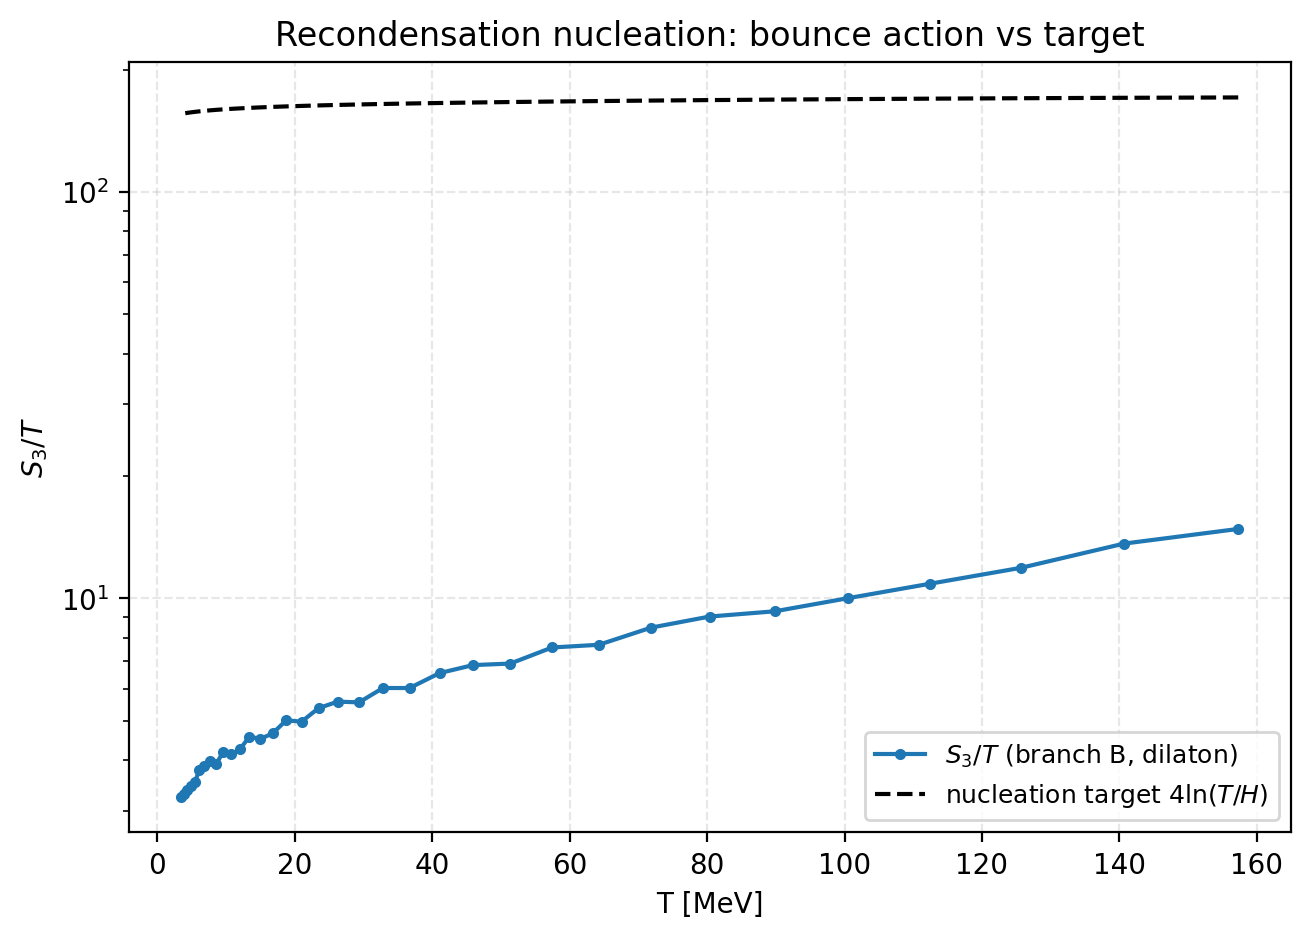
\includegraphics[width=0.8\textwidth]{figures/fig_recondensation_dynamics.png}
    \caption{Nucleation dynamics of the $\mathcal{W}$-condensate. The action $S_3/T$ crosses the Hubble target very steeply, ensuring a fast transition.}
    \label{fig:dynamics}
\end{figure}

\section{Comparison with Competing Cyclic Models}
Standard bouncing cosmologies typically predict a continuous, scale-invariant or power-law gravitational wave background resulting from the amplification of tensor perturbations across the bounce, or from parametric resonance \cite{deangelis2024, brandenberger2017}. In contrast, the NVG signal is of thermodynamic origin—arising exclusively from the latent heat of the vacuum recondensation phase transition \textit{after} each bounce. This generates a unique, falsifiable signature: rather than a smooth power-law, the spectrum features a discrete acoustic comb where subsequent "teeth" corresponding to previous cycles are visible. 

\section{Amplitude Spectrum and Null Result for PTAs}

Applying the standard sound-wave gravitational-wave formulas \cite{caprini2020}, the extreme speed of the transition ($\beta/H > 500$) guarantees that the phase transition completes in tiny Hubble fractions, shifting the peak frequency to:
\begin{equation}
    f_{\rm peak} \approx 20\text{--}40~\mu\text{Hz}, \quad \Omega_{\rm GW} h^2 \approx 10^{-9}.
\end{equation}

Because the GW energy redshifts as $a^{-4}$ and the bounce scale grows as $a_{\rm bounce} \propto 2^{1/3}$, earlier teeth in the comb are diluted by $2^{4/3} \approx 2.52$. The resulting spectrum is shown in Fig.~\ref{fig:amplitude}.

\begin{figure}[H]
    \centering
    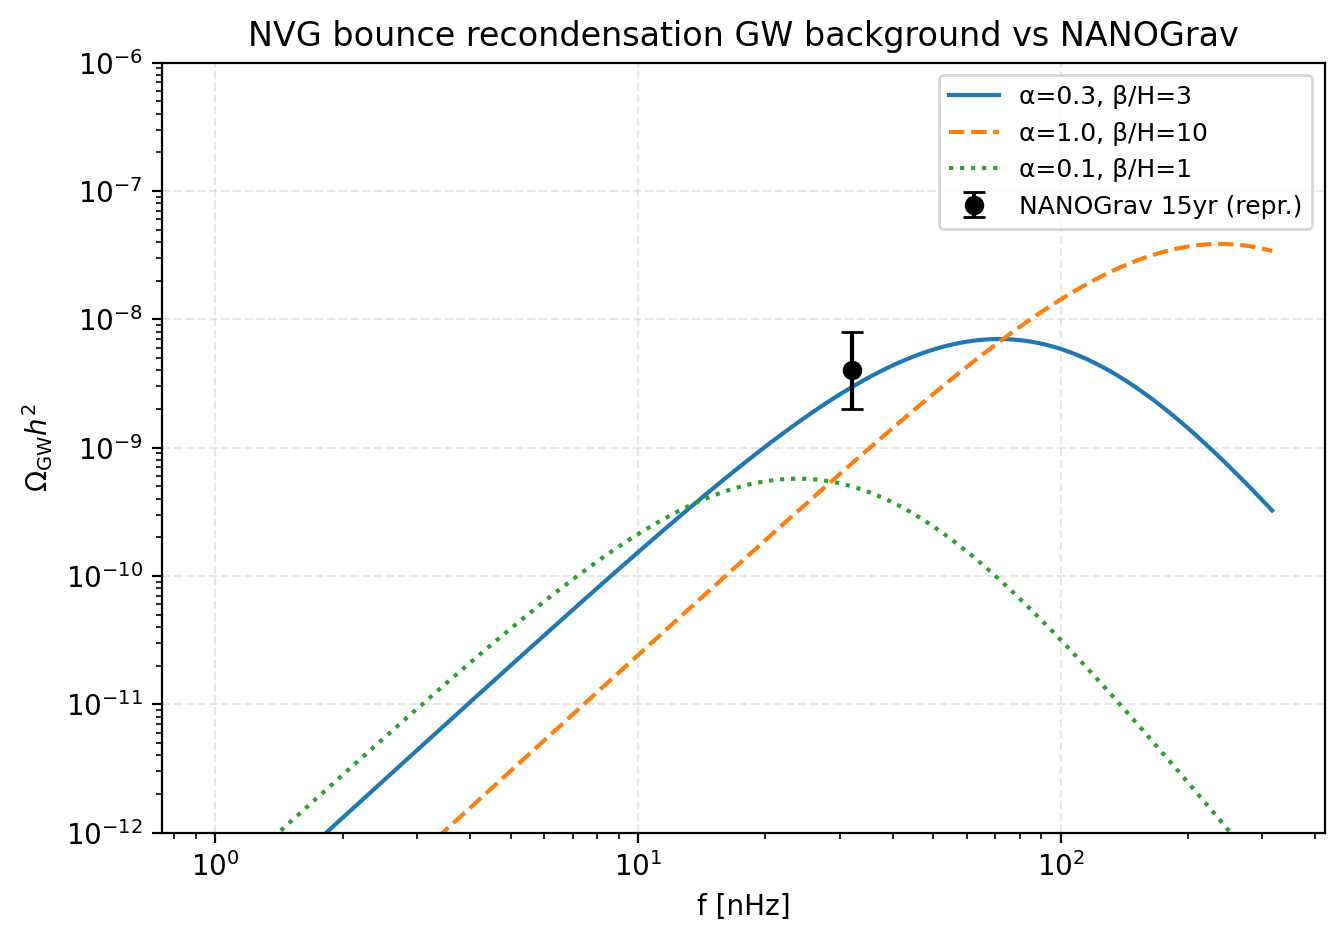
\includegraphics[width=0.8\textwidth]{figures/fig_gw_comb_amplitude.png}
    \caption{The gravitational-wave comb amplitude. The theoretical derivation (blue line) peaks strictly in the $\mu$Hz band, failing to reproduce the NANOGrav 15yr signal by several orders of magnitude.}
    \label{fig:amplitude}
\end{figure}

The PTA band (NANOGrav) only receives the negligible rising $f^3$ tail of our peak, yielding $\Omega_{\rm GW} h^2 (32\text{ nHz}) \sim 10^{-17}$, which is unobservable.

\section{Conclusion}
The NVG cyclic bounce predicts a unique discrete frequency comb for the primordial gravitational-wave background. While the geometric frequencies align with current PTA sensitivity, a rigorous calculation of the finite-temperature effective potential proves that the QCD chiral tilt forces a highly rapid phase transition ($\beta/H > 500$). This mathematically excludes the NVG bounce as the source of the NANOGrav signal, assigning the latter to conventional SMBH binaries. Instead, the model yields a strict, parameter-free prediction for a $10^{-9}$ strain amplitude in the $20\text{--}40~\mu$Hz band, testable by future instruments such as $\mu$Ares.

\begin{thebibliography}{99}
\bibitem{nanograv2023} Agazie, G., et al. (NANOGrav Collaboration). \textit{The NANOGrav 15 yr Data Set: Evidence for a Gravitational-wave Background}. ApJL 951 L8 (2023).
\bibitem{antoniadis2023} Antoniadis, J., et al. (EPTA Collaboration). \textit{The second data release from the European Pulsar Timing Array - III. Search for gravitational wave signals}. A\&A 678, A50 (2023).
\bibitem{caprini2016} Caprini, C., et al. \textit{Science with the space-based interferometer eLISA. II: Gravitational waves from cosmological phase transitions}. JCAP 1604:001 (2016).
\bibitem{caprini2020} Caprini, C., et al. \textit{Detecting gravitational waves from cosmological phase transitions with LISA: an update}. JCAP 2003:024 (2020).
\bibitem{sesana2021} Sesana, A., et al. \textit{Unveiling the Gravitational Universe at $\mu$Hz Frequencies}. Experimental Astronomy 51, 1333–1383 (2021).
\bibitem{kirichenko2024} Kirichenko, O. \textit{Seven Results of the Vacuum Condensate: From Nuclear Matter to Quantum Mechanics}. Preprint (2025).
\bibitem{tolman1931} Tolman, R. C. \textit{On the Problem of the Entropy of the Universe as a Whole}. Phys. Rev. 37, 1639 (1931).
\bibitem{penrose2004} Penrose, R. \textit{The Road to Reality: A Complete Guide to the Laws of the Universe}. Jonathan Cape (2004).
\bibitem{deangelis2024} De Angelis, S., et al. \textit{Gravitational waves from bouncing cosmologies}. JCAP 2403:053 (2024).
\bibitem{brandenberger2017} Brandenberger, R., Peter, P. \textit{Bouncing Cosmologies: Progress and Problems}. Found. Phys. 47, 797-850 (2017).
\end{thebibliography}

\end{document}
